FPGA-OpenCL - система автоматизации вычислений на FPGA-ускорителях на основе
 стандарта OpenCL. В неё входят следующие компоненты:
\begin{enumerate}
   \item Реализация некоторого подмножества OpenCL достаточного для работы с
   FPGA.
   \item Механизм обмена данными.
   \item Диспетчер запросов на выполнение команд на акселераторе.
   \item Драйвер для осуществления взаимодействия между устройством и
   центральным процессором.
   \item Генерация прошивки для устройства на основе созданных OpenCL ядер.
\end{enumerate}

Общая схема работы FPGA-OpenCL:

\begin{figure}[h!]
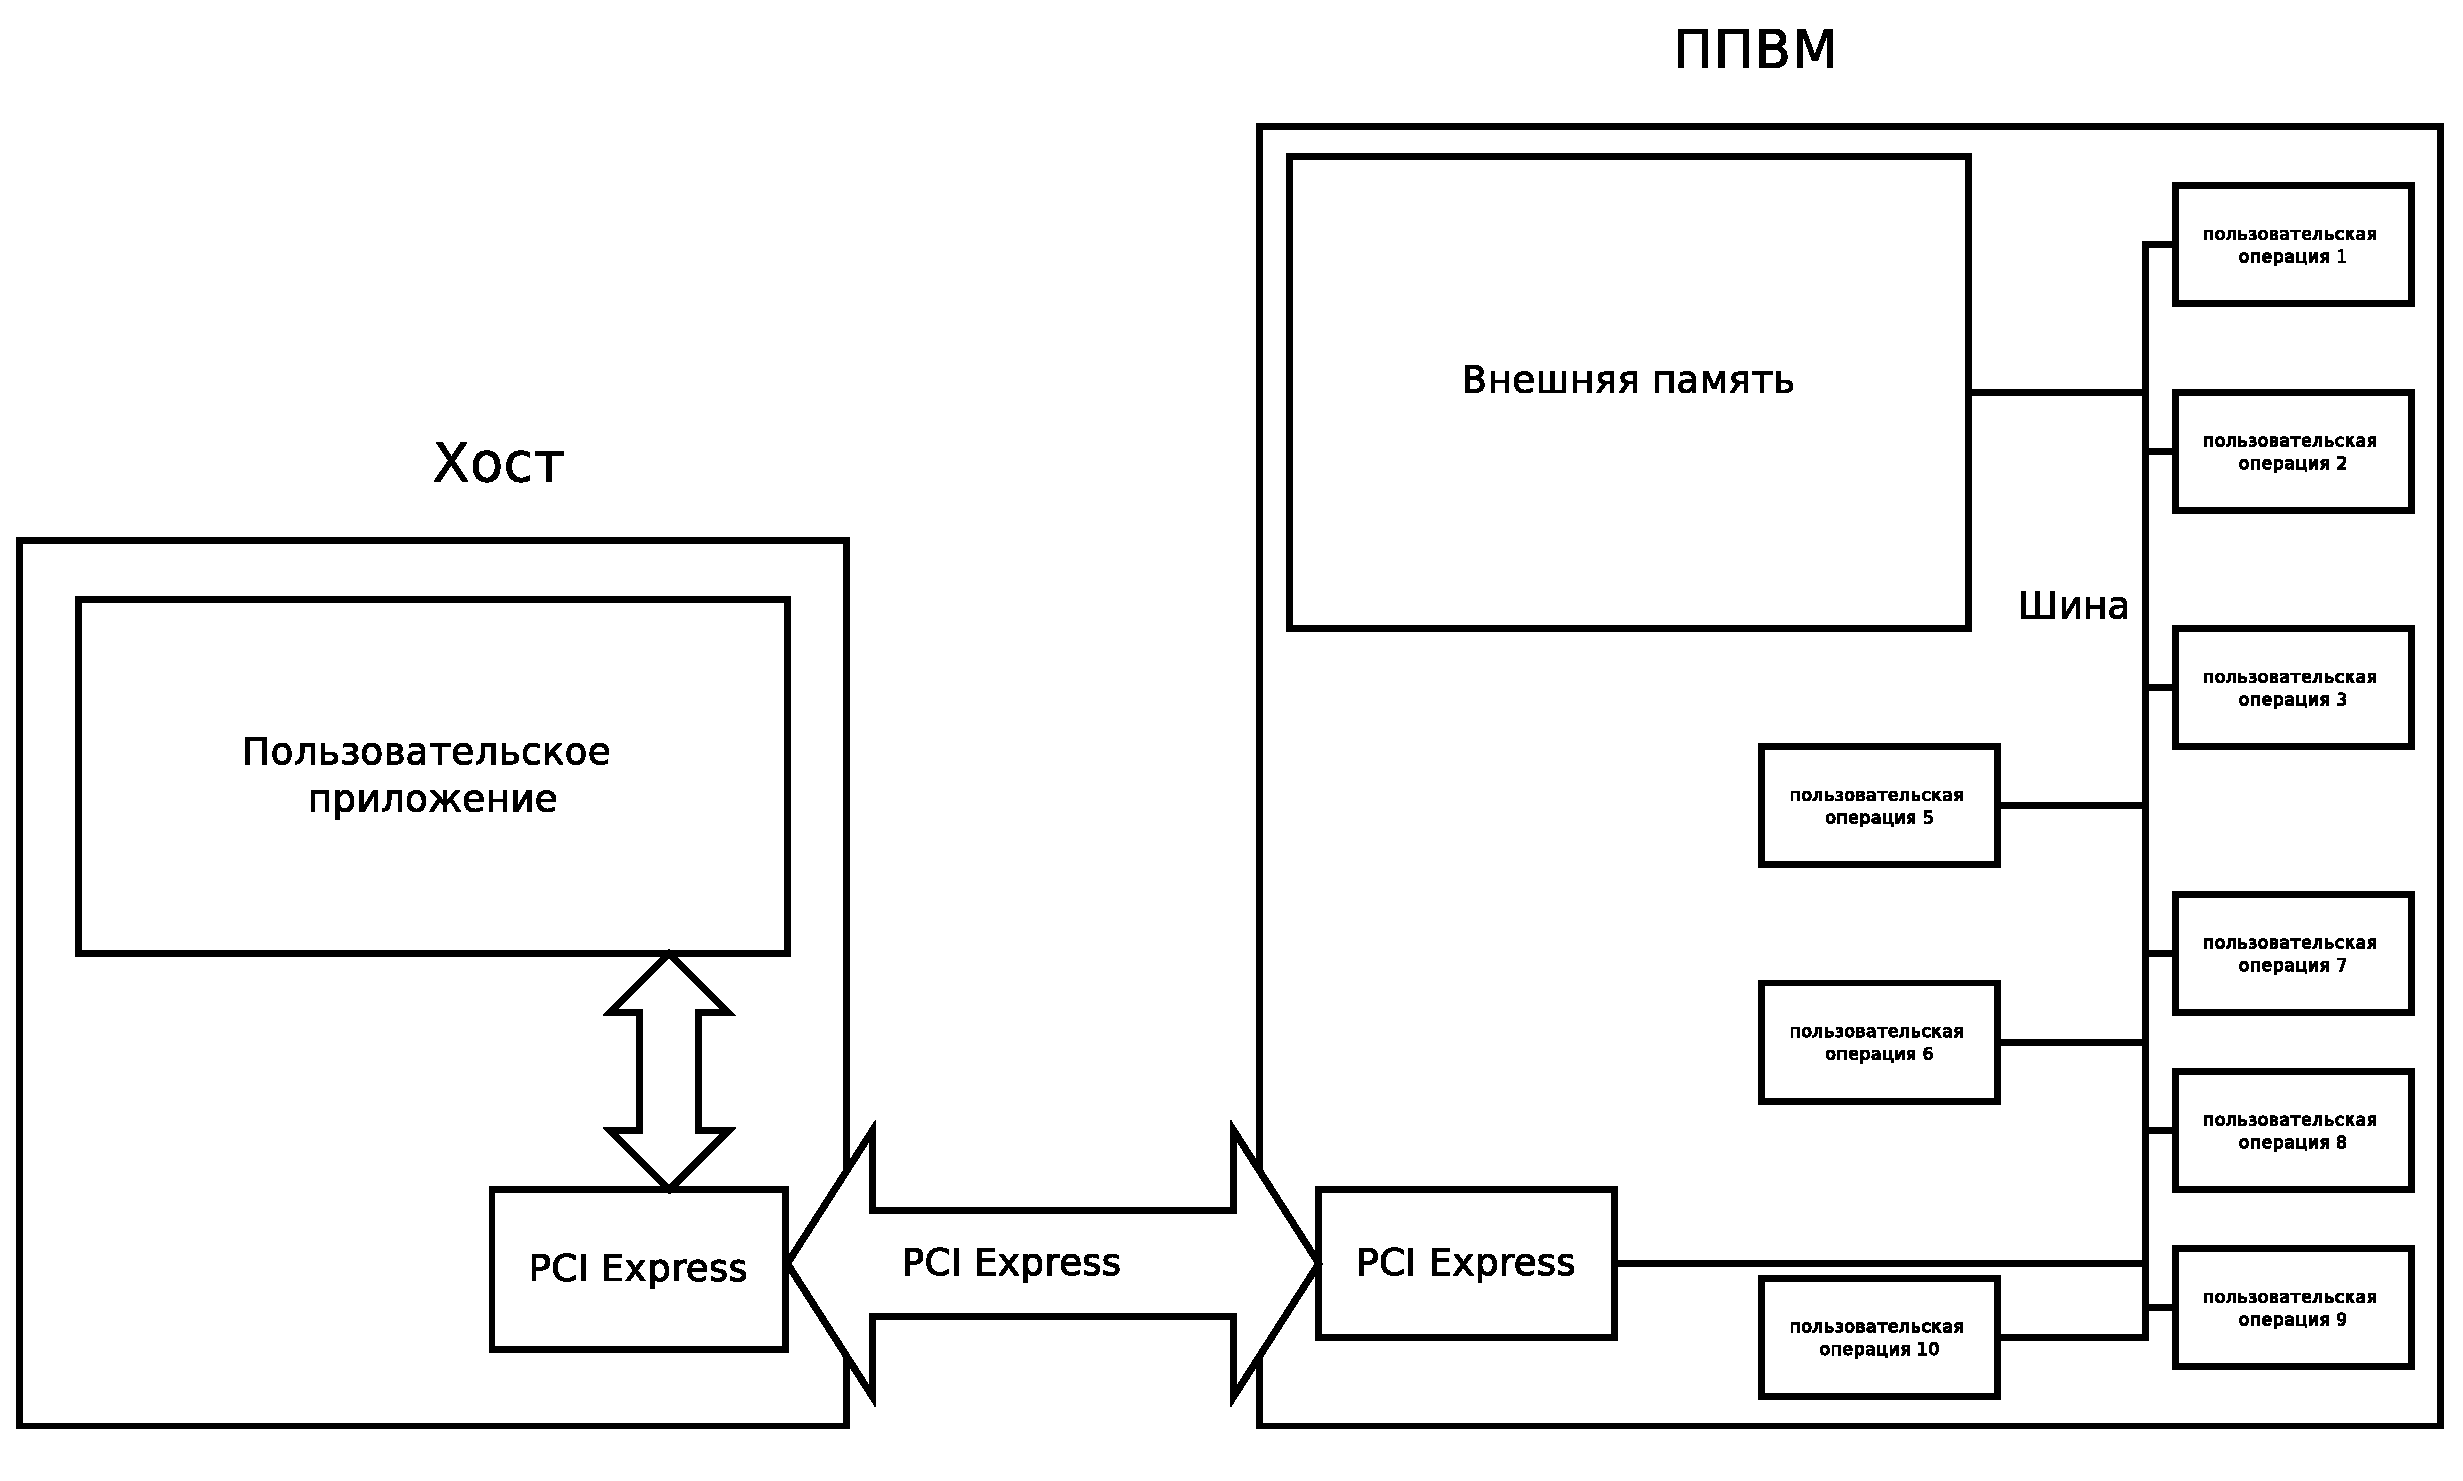
\includegraphics [width=\textwidth]{pictures/base-scheme}
\caption{Общая схема работы FPGA-OpenCL}
\label{fpga-cell}
\end{figure}

В рамках данной работы были произведены две реализации диспетчера задач. Первая
реализация работала на софтверном процессоре акселератора, вторая была размещена
непосредственно в драйвере.
